%%%%%%%%%%%%%%%%%%%%%%%%%%%%%%%%%%%%%%%%%%%%%%%%%%%%%%%%%%%%%%%%%%%%%%%%%%%%%%%%%%
\begin{frame}[fragile]\frametitle{}
\begin{center}
{\Large Logistic Regression with Scikit-Learn}
\end{center}
\end{frame}


%%%%%%%%%%%%%%%%%%%%%%%%%%%%%%%%%%%%%%%%%%%%%%%%%%%%%%%%%%%%%%%%%%%%%%%%
\begin{frame}[fragile]\frametitle{Logistic Regression}
\begin{lstlisting}
# Logistic Regression
from sklearn import datasets
from sklearn import metrics
from sklearn.linear_model import LogisticRegression
# load the iris datasets
dataset = datasets.load_iris()
# fit a logistic regression model to the data
model = LogisticRegression()
model.fit(dataset.data, dataset.target)
print(model)
# make predictions
expected = dataset.target
predicted = model.predict(dataset.data)
# summarize the fit of the model
print(metrics.classification_report(expected, predicted))
print(metrics.confusion_matrix(expected, predicted))
\end{lstlisting}

{\tiny (Ref: Machine Learning Algorithm Recipes in scikit-learn - Jason Brownlee)}

\end{frame}



% %%%%%%%%%%%%%%%%%%%%%%%%%%%%%%%%%%%%%%%%%%%%%%%%%%%%%%%%%%%%%%%%%%%%%%%%
% \begin{frame}[fragile]\frametitle{Template of Logistic Regression}
% Logistic regression is available in scikit-learn
% \begin{lstlisting}
% from sklearn.linear_model import LogisticRegression 

% # Assumed you have, X (predictor) and Y (target) 
% # for training data set and x_test(predictor) of test_dataset 

% model = LogisticRegression() 

% model.fit(X, y) 

% model.score(X, y) 

% print('Coefficient: \n', model.coef_) 
% print('Intercept: \n', model.intercept_) 

% predicted= model.predict(x_test) 
% \end{lstlisting}

% \end{frame}

% %%%%%%%%%%%%%%%%%%%%%%%%%%%%%%%%%%%%%%%%%%%%%%%%%%%%%%%%%%%%%%%%%%%%%%%%%%%%%%%%%%
% \begin{frame}[fragile]\frametitle{}
% \begin{center}
% {\Large Test case: Iris Flowers}
% \end{center}
% \end{frame}


% %%%%%%%%%%%%%%%%%%%%%%%%%%%%%%%%%%%%%%%%%%%%%%%%%%%%%%%%%%%%%%%%%%%%%%%%
% \begin{frame}[fragile]\frametitle{Load Iris Data}
% \begin{lstlisting}
% import pandas as pd
% iris  = pd.read_csv(`data/iris.csv')
% print(iris.head())
% \end{lstlisting}
% \begin{center}
% 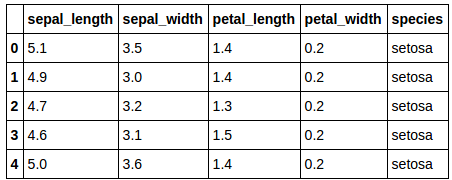
\includegraphics[width=0.8\linewidth,keepaspectratio]{irishead}
% \end{center}
% \end{frame}

% % %%%%%%%%%%%%%%%%%%%%%%%%%%%%%%%%%%%%%%%%%%%%%%%%%%%%%%%%%%%%%%%%%%%%%%%%
% % \begin{frame}[fragile]\frametitle{Describe Iris Data}

% % \begin{lstlisting}
   % % sepal_length_cm  sepal_width_cm  petal_length_cm  petal_width_cm  \
% % 0              5.1             3.5              1.4             0.2   
% % 1              4.9             3.0              1.4             0.2   
% % 2              4.7             3.2              1.3             0.2   
% % 3              4.6             3.1              1.5             0.2   
% % 4              5.0             3.6              1.4             0.2   

         % % class  
% % 0  Iris-setosa  
% % 1  Iris-setosa  
% % 2  Iris-setosa  
% % 3  Iris-setosa  
% % 4  Iris-setosa  
% % \end{lstlisting}


% % \end{frame}

% %%%%%%%%%%%%%%%%%%%%%%%%%%%%%%%%%%%%%%%%%%%%%%%%%%%%%%%%%%%%%%%%%%%%%%%%
% \begin{frame}[fragile]\frametitle{Describe Iris Data}
% \begin{center}
% 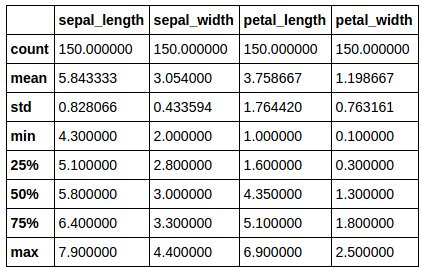
\includegraphics[width=0.8\linewidth,keepaspectratio]{irisdescribe}
% \end{center}
% \end{frame}

% %%%%%%%%%%%%%%%%%%%%%%%%%%%%%%%%%%%%%%%%%%%%%%%%%%%%%%%%%%%%%%%%%%%%%%%%
% \begin{frame}[fragile]\frametitle{Visualize Data}
% \begin{center}
% 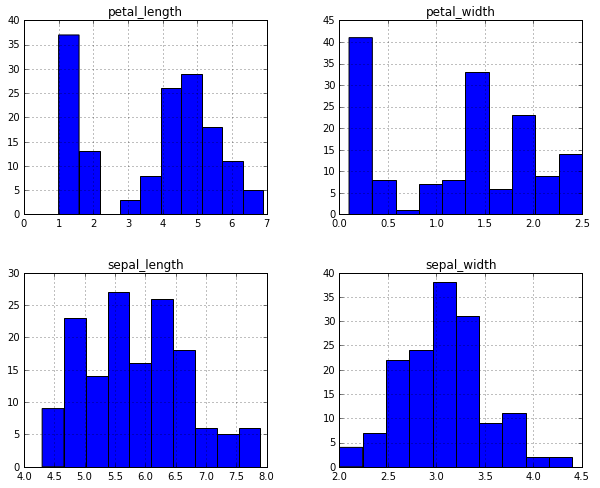
\includegraphics[width=0.8\linewidth,keepaspectratio]{irishist}
% \end{center}
% \end{frame}

% %%%%%%%%%%%%%%%%%%%%%%%%%%%%%%%%%%%%%%%%%%%%%%%%%%%%%%%%%%%%%%%%%%%%%%%%%
% %\begin{frame}[fragile]\frametitle{Setup Plotting}
% %\begin{lstlisting}
% %
% %\end{lstlisting}
% %\end{frame}


% %%%%%%%%%%%%%%%%%%%%%%%%%%%%%%%%%%%%%%%%%%%%%%%%%%%%%%%%%%%%%%%%%%%%%%%%
% \begin{frame}[fragile]\frametitle{Scatter Plot}
% \begin{itemize}
% \item The first way we can plot things is using the .plot extension from Pandas dataframes
% \item We'll use this to make a scatterplot of the Iris features.
% \end{itemize}
% \begin{lstlisting}
% import seaborn as sns
% import matplotlib.pyplot as plt
% sns.set(style="white", color_codes=True)

% iris.plot(kind="scatter", x="sepal_length_cm", y="sepal_width_cm")
% plt.show()
% \end{lstlisting}
% Plot?
% \end{frame}

% %%%%%%%%%%%%%%%%%%%%%%%%%%%%%%%%%%%%%%%%%%%%%%%%%%%%%%%%%%%%%%%%%%%%%%%%
% \begin{frame}[fragile]\frametitle{Scatter Plot}
% \begin{center}
% 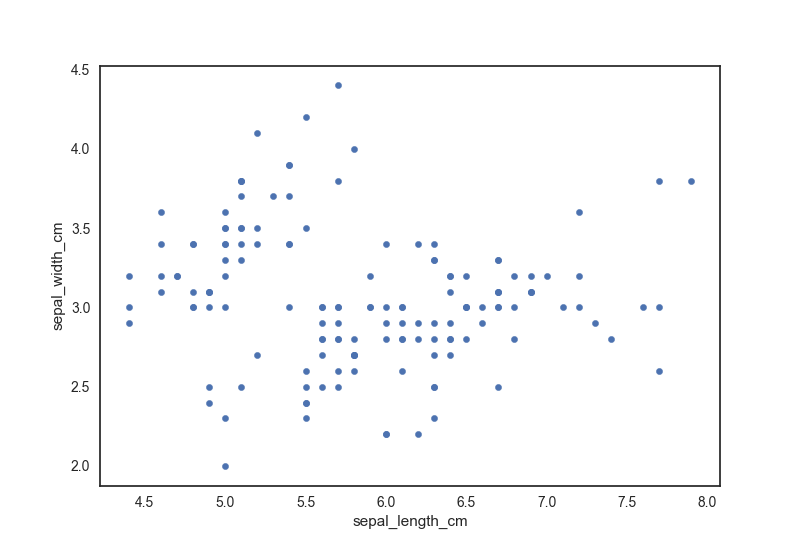
\includegraphics[width=\linewidth,keepaspectratio]{irisscatter1}
% \end{center}
% \end{frame}


% %%%%%%%%%%%%%%%%%%%%%%%%%%%%%%%%%%%%%%%%%%%%%%%%%%%%%%%%%%%%%%%%%%%%%%%%
% \begin{frame}[fragile]\frametitle{Facet Grid}
% \begin{itemize}
% \item One piece of information missing in the plots above is what species each plant is
% \item We'll use seaborn's FacetGrid to color the scatterplot by species
% \end{itemize}
% \begin{lstlisting}
% sns.FacetGrid(iris, hue="Species", size=5) \
   % .map(plt.scatter, "sepal_length_cm", "sepal_width_cm") \
   % .add_legend()

% plt.show()
% \end{lstlisting}
% Plot?
% \end{frame}

% %%%%%%%%%%%%%%%%%%%%%%%%%%%%%%%%%%%%%%%%%%%%%%%%%%%%%%%%%%%%%%%%%%%%%%%%
% \begin{frame}[fragile]\frametitle{FacetGrid Plot}
% \begin{center}
% 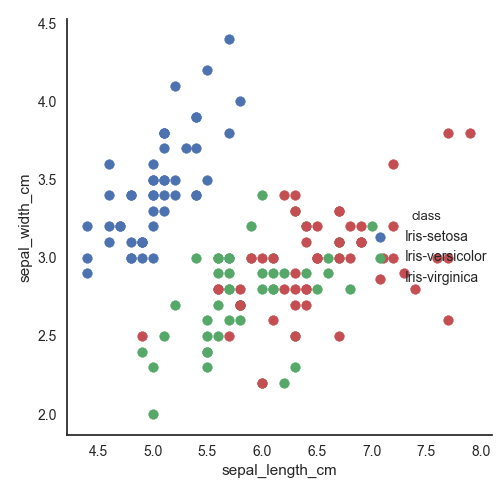
\includegraphics[width=0.7\linewidth,keepaspectratio]{irisscatter2}
% \end{center}
% \end{frame}

% %%%%%%%%%%%%%%%%%%%%%%%%%%%%%%%%%%%%%%%%%%%%%%%%%%%%%%%%%%%%%%%%%%%%%%%%
% \begin{frame}[fragile]\frametitle{Box Plot}
% \begin{itemize}
% \item We can look at an individual feature in Seaborn through a boxplot
% \end{itemize}
% \begin{lstlisting}
% sns.boxplot(x="class", y="petal_length_cm", data=iris)
% \end{lstlisting}
% Plot?
% \end{frame}


% %%%%%%%%%%%%%%%%%%%%%%%%%%%%%%%%%%%%%%%%%%%%%%%%%%%%%%%%%%%%%%%%%%%%%%%%
% \begin{frame}[fragile]\frametitle{Box Plot}
% \begin{center}
% 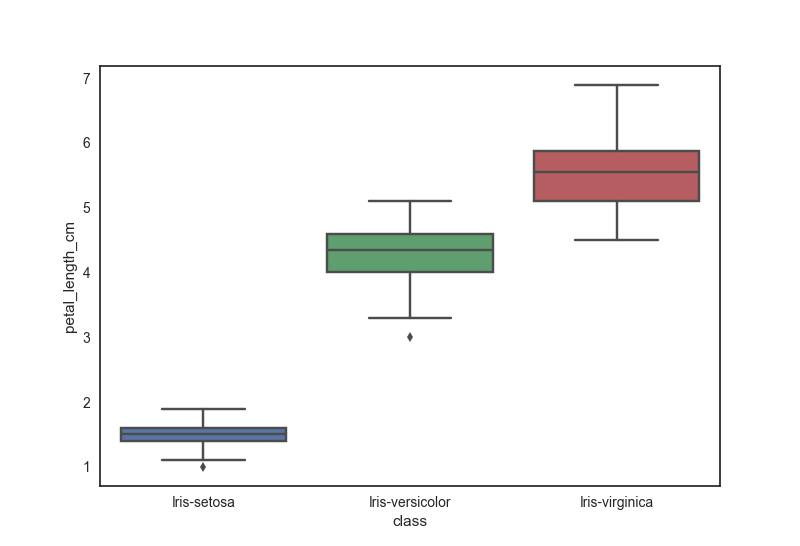
\includegraphics[width=\linewidth,keepaspectratio]{irisscatter3}
% \end{center}
% \end{frame}

% %%%%%%%%%%%%%%%%%%%%%%%%%%%%%%%%%%%%%%%%%%%%%%%%%%%%%%%%%%%%%%%%%%%%%%%%
% \begin{frame}[fragile]\frametitle{Pairs Plot}
% \begin{itemize}
% \item Bivariate relation between each pair of features
% \item From the pairplot, we'll see that the Iris-setosa species is separataed from the other two across all feature combinations
% \end{itemize}
% \begin{lstlisting}
% sns.pairplot(iris, hue="class", size=3)
% \end{lstlisting}
% Plot?
% \end{frame}

% %%%%%%%%%%%%%%%%%%%%%%%%%%%%%%%%%%%%%%%%%%%%%%%%%%%%%%%%%%%%%%%%%%%%%%%%
% \begin{frame}[fragile]\frametitle{Pairs Plot}
% \begin{center}
% 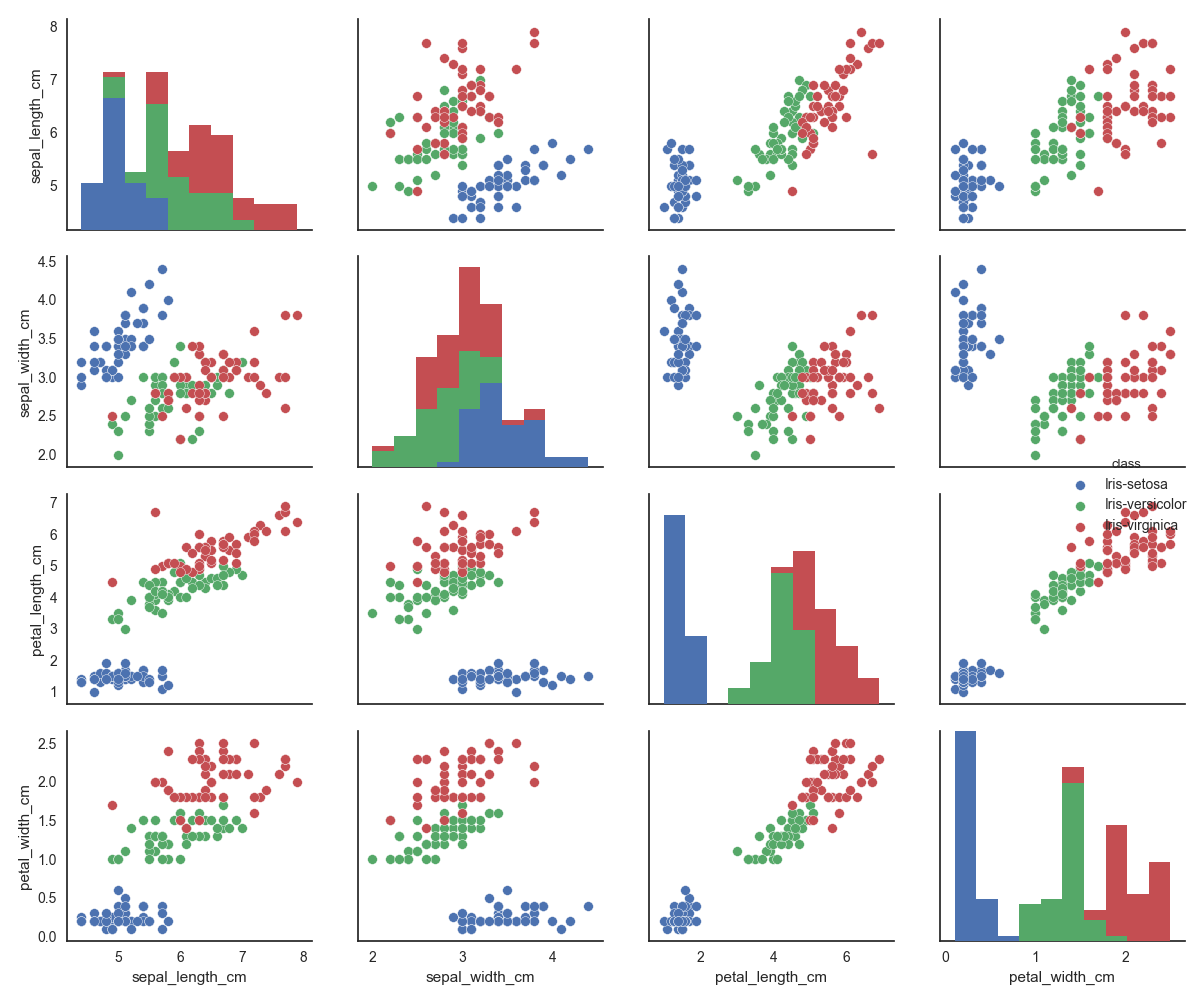
\includegraphics[width=0.8\linewidth,keepaspectratio]{irisscatter4}
% \end{center}
% \end{frame}


% %%%%%%%%%%%%%%%%%%%%%%%%%%%%%%%%%%%%%%%%%%%%%%%%%%%%%%%%%%%%%%%%%%%%%%%%
% \begin{frame}[fragile]\frametitle{Encode The Output Variable}
% The output variable contains three different string values.
% \begin{lstlisting}
% Iris-setosa
% Iris-versicolor
% Iris-virginica
% \end{lstlisting}

% We can turn these into integers. We cannot use One-hot encoding dummies here, as we need only one output column:
% \begin{lstlisting}
% iris['Species'] = iris['Species'].map({'Iris-setosa':0,'Iris-versicolor':1,'Iris-virginica':2})
% \end{lstlisting}


% % We can turn this into a one-hot encoded binary matrix for each data instance that would look as follows:
% % \begin{lstlisting}
% % # encode class values as integers
% % encoder = LabelEncoder()
% % encoder.fit(Y)
% % encoded_Y = encoder.transform(Y)
% % # convert integers to dummy variables (i.e. one hot encoded)
% % dummy_y = np_utils.to_categorical(encoded_Y)
% % \end{lstlisting}
% Print the output.
% \end{frame}

% %%%%%%%%%%%%%%%%%%%%%%%%%%%%%%%%%%%%%%%%%%%%%%%%%%%%%%%%%%%%%%%%%%%%%%%%
% \begin{frame}[fragile]\frametitle{Prep Training Data - Manual way}
% \begin{itemize}
% \item We can then split the attributes (columns) into input variables (X) and output variables (Y).
% \end{itemize}
% \begin{lstlisting}
% dataset = iris.values
% X = dataset[:,0:4].astype(float)
% Y = dataset[:,4]
% \end{lstlisting}
% \end{frame}


% %%%%%%%%%%%%%%%%%%%%%%%%%%%%%%%%%%%%%%%%%%%%%%%%%%%%%%%%%%%%%%%%%%%%%%%%
% \begin{frame}[fragile]\frametitle{Prep Training Data - Ready way}
% Iris dataset is READILY available as csv also as part of sklearn
% \begin{lstlisting}
% from sklearn.linear_model import LogisticRegression
% from sklearn import datasets

% iris = datasets.load_iris()

% # Assign petal length and petal width to X matrix (150 samples)
% X = iris.data[:, [2, 3]]

% # Class labels
% y = iris.target
% \end{lstlisting}

% \end{frame}

% %%%%%%%%%%%%%%%%%%%%%%%%%%%%%%%%%%%%%%%%%%%%%%%%%%%%%%%%%%%%%%%%%%%%%%%%
% \begin{frame}[fragile]\frametitle{Iris: Logistic Regression}
% \begin{lstlisting}
% # Split the dataset into separate training and test datasets.
% from sklearn.model_selection.cross_validation import train_test_split

% # Split the X and y arrays into 30 percent test data, and 70 (45 samples) percent training data (105 samples)
% X_train, X_test, y_train, y_test = train_test_split(X, y, test_size=0.3, random_state=0)
% \end{lstlisting}

% \end{frame}

% %%%%%%%%%%%%%%%%%%%%%%%%%%%%%%%%%%%%%%%%%%%%%%%%%%%%%%%%%%%%%%%%%%%%%%%%
% \begin{frame}[fragile]\frametitle{Iris: Logistic Regression}
% \begin{lstlisting}
% # Optimization - Feature scaling
% from sklearn.preprocessing import StandardScaler

% # Initlalize a new StandardScaler object, sc
% sc = StandardScaler()

% # Using the fit method, estimate the sample mean and standard deviation for each feature dimension. 
% sc.fit(X_train)

% # Transform both training and test sets using the sample mean and standard deviations
% X_train_std = sc.transform(X_train)
% X_test_std = sc.transform(X_test)

% X_combined_std = np.vstack((X_train_std, X_test_std))
% y_combined = np.hstack((y_train, y_test))
% \end{lstlisting}

% \end{frame}

% %%%%%%%%%%%%%%%%%%%%%%%%%%%%%%%%%%%%%%%%%%%%%%%%%%%%%%%%%%%%%%%%%%%%%%%%
% \begin{frame}[fragile]\frametitle{Iris: Logistic Regression}
% \begin{lstlisting}
% lr = LogisticRegression()
% lr.fit(X_train, y_train)

% \end{lstlisting}

% \end{frame}

% % %%%%%%%%%%%%%%%%%%%%%%%%%%%%%%%%%%%%%%%%%%%%%%%%%%%%%%%%%%%%%%%%%%%%%%%%
% % \begin{frame}[fragile]\frametitle{Iris: Logistic Regression}
% % \begin{lstlisting}
% % lr = LogisticRegression(C=1000.0, random_state=0)

% % lr.fit(X_train_std, y_train)

% % plot_decision_regions(X_combined_std, y_combined, classifier=lr, test_idx=range(105,150))

% % plt.xlabel('petal length [standardized]')
% % plt.ylabel('petal width [standardized]')
% % plt.legend(loc='upper left')
% % plt.show()
% % \end{lstlisting}

% % \end{frame}

% % %%%%%%%%%%%%%%%%%%%%%%%%%%%%%%%%%%%%%%%%%%%%%%%%%%%%%%%%%%%%%%%%%%%%%%%%
% % \begin{frame}[fragile]\frametitle{Iris: Logistic Regression}
% % \begin{center}
% % 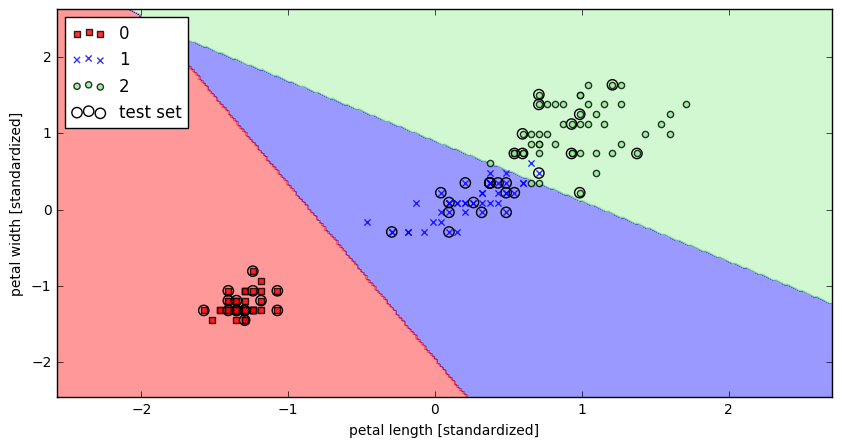
\includegraphics[width=0.9\linewidth]{irislog}
% % \end{center}
% % \end{frame}


% % %%%%%%%%%%%%%%%%%%%%%%%%%%%%%%%%%%%%%%%%%%%%%%%%%%%%%%%%%%%%%%%%%%%%%%%%
% % \begin{frame}[fragile]\frametitle{Iris: Tackling overfitting via regularization}
	% % \begin{itemize}
	% % \item Overfitting, high variance (variability, sensitive to randomness in the data). Model performs well on seen data.
  	% % \item  Underfitting, high bias (measure of the systematic error that is not due to randomness). Model performs low on unseen data.
	% % \item 
   % % Regularization is a usefull method to handle collinearity (high correlation among features), filter out noise from data, and eventually prevent overfitting.
   	% % \item To make sure regularization works properly, ensure that all features are on a comparable scale (feature scaling standardization)

	% % \end{itemize}
% % \end{frame}

% % %%%%%%%%%%%%%%%%%%%%%%%%%%%%%%%%%%%%%%%%%%%%%%%%%%%%%%%%%%%%%%%%%%%%%%%%
% % \begin{frame}[fragile]\frametitle{Iris: Tackling over-fitting via regularization}
	% % \begin{itemize}
	% % \item In regularization, apart from cost function, weighted sum of parameters and features is added
	% % \item For the features which need to be suppressed, their corresponding coefficient is made large. So their cost component increases
	% % \item As the Cost needs to be minimized, to reduce these weighted sum, corresponding feature values are reduced, 
	% % \item So their importances gets lowered dramatically.

	% % \end{itemize}
% % \end{frame}


% % %%%%%%%%%%%%%%%%%%%%%%%%%%%%%%%%%%%%%%%%%%%%%%%%%%%%%%%%%%%%%%%%%%%%%%%%
% % \begin{frame}[fragile]\frametitle{Iris: Tackling over-fitting via regularization}
% % The figure below, you can see that the weight coefficients shrink if we decrease the parameter C, that is, when we increase the regularization strength
% % \begin{lstlisting}
% % weights, params = [], []

% % for c in np.arange(-5, 5):
   % % lr = LogisticRegression(C=10**c, random_state=0)
   % % lr.fit(X_train_std, y_train)
   % % weights.append(lr.coef_[1])
   % % params.append(10**c)

% % weights = np.array(weights)
% % plt.plot(params, weights[:, 0], label='petal length')
% % plt.plot(params, weights[:, 1], linestyle='--', label='petal width')
% % plt.ylabel('weight coefficient')
% % plt.xlabel('C')
% % plt.legend(loc='upper left')
% % plt.xscale('log')
% % plt.show()
% % \end{lstlisting}
% % \end{frame}

% % %%%%%%%%%%%%%%%%%%%%%%%%%%%%%%%%%%%%%%%%%%%%%%%%%%%%%%%%%%%%%%%%%%%%%%%%
% % \begin{frame}[fragile]\frametitle{Iris: Logistic Regression}
% % \begin{center}
% % 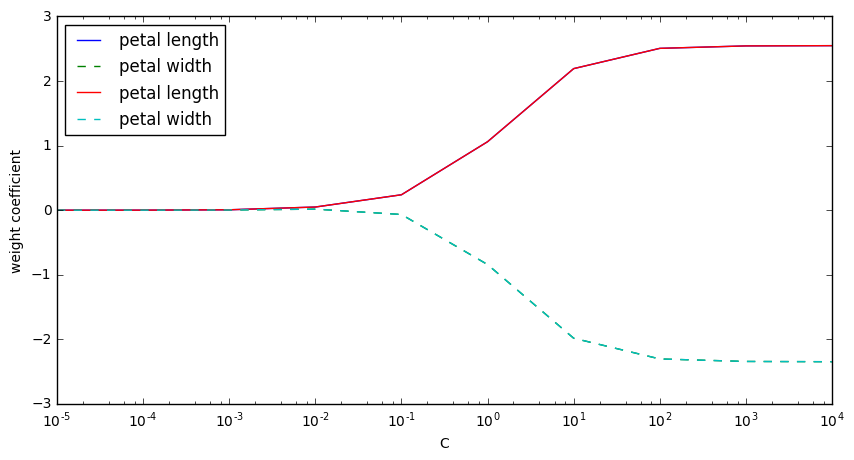
\includegraphics[width=0.9\linewidth]{irisreg}
% % \end{center}
% % \end{frame}

% %%%%%%%%%%%%%%%%%%%%%%%%%%%%%%%%%%%%%%%%%%%%%%%%%%%%%%%%%%%%%%%%%%%%%%%%%%%%%%%%%%
% \begin{frame}[fragile]\frametitle{}
% \begin{center}
% {\Large Test case: Glass Identification}
% \end{center}
% \end{frame}

% %%%%%%%%%%%%%%%%%%%%%%%%%%%%%%%%%%%%%%%%%%%%%%%%%%%%%%%%%%%%%%%%%%%%%%%%
% \begin{frame}[fragile]\frametitle{Glass identification Dataset}
% Location: http://archive.ics.uci.edu/ml/machine-learning-databases/glass/glass.data
% \begin{lstlisting}
% import pandas as pd
% col_names = ['id','ri','na','mg','al','si','k','ca','ba','fe','glass_type']
% glass = pd.read_csv('glass.data', names=col_names, index_col='id')

% glass.sort('al', inplace=True)
% print(glass.head())
% \end{lstlisting}
% \end{frame}


% %%%%%%%%%%%%%%%%%%%%%%%%%%%%%%%%%%%%%%%%%%%%%%%%%%%%%%%%%%%%%%%%%%%%%%%%
% \begin{frame}[fragile]\frametitle{Glass identification Dataset}
% \begin{center}
% 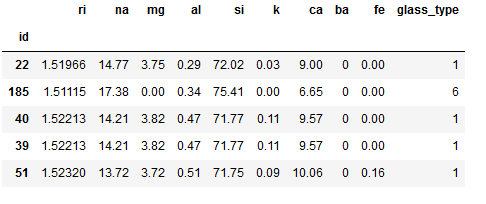
\includegraphics[width=0.8\linewidth]{glassdt}
% \end{center}
% % \tiny
% \begin{itemize}
% \item Question: Pretend that we want to predict glass type, and our only feature is al. How could we do it using machine learning?
% \item Answer: We could frame it as a classification problem, and use a logistic regression model with al as the only feature and glass type as the response.
% \end{itemize}
% \end{frame}


% %%%%%%%%%%%%%%%%%%%%%%%%%%%%%%%%%%%%%%%%%%%%%%%%%%%%%%%%%%%%%%%%%%%%%%%%
% \begin{frame}[fragile]\frametitle{Predicting a Categorical Response}
% \begin{lstlisting}
% # examine glass_type how many of each type
% print(glass.glass_type.value_counts().sort_index())
% 1    70
% 2    76
% 3    17
% 5    13
% 6     9
% 7    29
% # types 1, 2, 3 are window glass,
% # types 5, 6, 7 are household glass
% glass['household'] = glass.glass_type.map({1:0, 2:0, 3:0, 5:1, 6:1, 7:1})
% print(glass.head())
% \end{lstlisting}
% \end{frame}

% %%%%%%%%%%%%%%%%%%%%%%%%%%%%%%%%%%%%%%%%%%%%%%%%%%%%%%%%%%%%%%%%%%%%%%%%
% \begin{frame}[fragile]\frametitle{Predicting a Categorical Response}
% \begin{center}
% 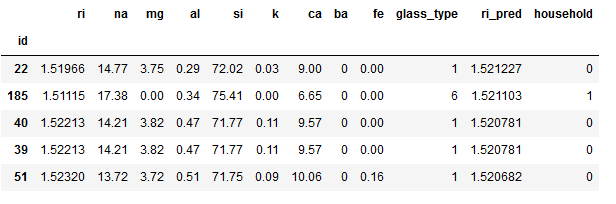
\includegraphics[width=0.9\linewidth]{glasstp}
% \end{center}
% \end{frame}

% %%%%%%%%%%%%%%%%%%%%%%%%%%%%%%%%%%%%%%%%%%%%%%%%%%%%%%%%%%%%%%%%%%%%%%%%
% \begin{frame}[fragile]\frametitle{Predicting a Categorical Response}
% We want to `household' using `al'. Let's visualize the relationship to figure out how to do this:
% \begin{lstlisting}
% plt.scatter(glass.al, glass.household)
% plt.xlabel('al')
% plt.ylabel('household')
% \end{lstlisting}
% \end{frame}

% %%%%%%%%%%%%%%%%%%%%%%%%%%%%%%%%%%%%%%%%%%%%%%%%%%%%%%%%%%%%%%%%%%%%%%%%
% \begin{frame}[fragile]\frametitle{Predicting a Categorical Response}

% \begin{center}
% 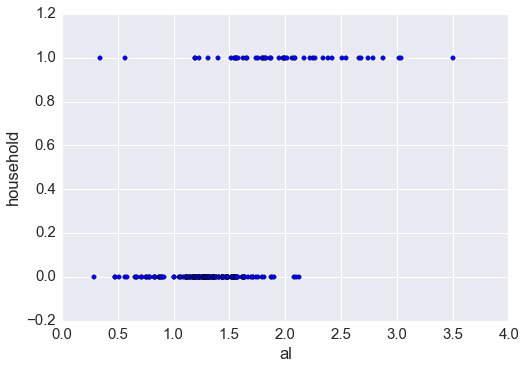
\includegraphics[width=0.9\linewidth]{glasshld}
% \end{center}
% \end{frame}


% %%%%%%%%%%%%%%%%%%%%%%%%%%%%%%%%%%%%%%%%%%%%%%%%%%%%%%%%%%%%%%%%%%%%%%%%
% \begin{frame}[fragile]\frametitle{Binary outcome}
% There is clear separation, almost like binary partition, Vertically!!!
% \begin{lstlisting}
% from sklearn.linear_model import LogisticRegression

% logreg = LogisticRegression(C=1e9)
% feature_cols = ['al']
% X = glass[feature_cols]
% y = glass.household
% logreg.fit(X, y)
% glass['household_pred_class'] = logreg.predict(X)

% plt.scatter(glass.al, glass.household)
% plt.plot(glass.al, glass.household_pred_class, color='red')
% \end{lstlisting}
% \end{frame}

% %%%%%%%%%%%%%%%%%%%%%%%%%%%%%%%%%%%%%%%%%%%%%%%%%%%%%%%%%%%%%%%%%%%%%%%%
% \begin{frame}[fragile]\frametitle{Binary outcome}
% \begin{center}
% 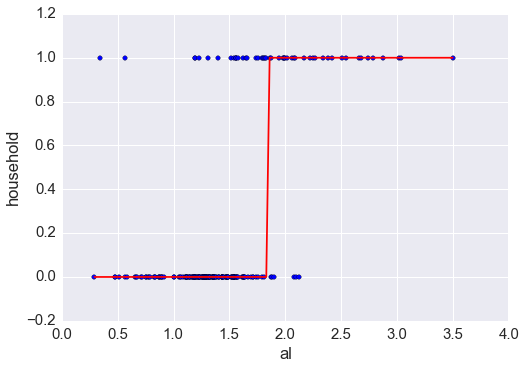
\includegraphics[width=0.9\linewidth]{glasshldplt}
% \end{center}
% \end{frame}

% %%%%%%%%%%%%%%%%%%%%%%%%%%%%%%%%%%%%%%%%%%%%%%%%%%%%%%%%%%%%%%%%%%%%%%%%
% \begin{frame}[fragile]\frametitle{Probability Prediction}
% What if we wanted the predicted probabilities instead of just the class predictions, to understand how confident we are in a given prediction?
% \begin{lstlisting}
% # store the predicted probabilites of class 1
% glass['household_pred_prob'] = logreg.predict_proba(X)[:, 1]
% # plot the predicted probabilities
% plt.scatter(glass.al, glass.household)
% plt.plot(glass.al, glass.household_pred_prob, color='red')
% plt.xlabel('al')
% plt.ylabel('household')
% \end{lstlisting}
% \end{frame}


% %%%%%%%%%%%%%%%%%%%%%%%%%%%%%%%%%%%%%%%%%%%%%%%%%%%%%%%%%%%%%%%%%%%%%%%%
% \begin{frame}[fragile]\frametitle{Probability Prediction}
% \begin{center}
% 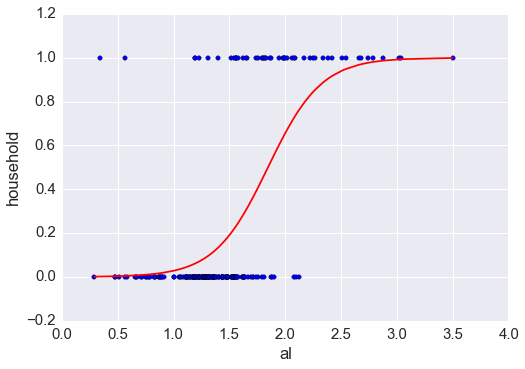
\includegraphics[width=0.9\linewidth]{glasshldpltprob}
% \end{center}
% \end{frame}


% %%%%%%%%%%%%%%%%%%%%%%%%%%%%%%%%%%%%%%%%%%%%%%%%%%%%%%%%%%%%%%%%%%%%%%%%
% \begin{frame}[fragile]\frametitle{Probability Prediction}

% \begin{lstlisting}
% # examine some example predictions
% print(logreg.predict_proba(1))
% print(logreg.predict_proba(2))
% print(logreg.predict_proba(3))

% [[ 0.97161726  0.02838274]]
% [[ 0.34361555  0.65638445]]
% [[ 0.00794192  0.99205808]]
% \end{lstlisting}
% The first column indicates the predicted probability of class 0, and the second column indicates the predicted probability of class 1.
% \end{frame}

% %
% %%%%%%%%%%%%%%%%%%%%%%%%%%%%%%%%%%%%%%%%%%%%%%%%%%%%%%%%%%%%%%%%%%%%%%%%%
% %\begin{frame}[fragile]\frametitle{Using Logistic Regression with Categorical Features}
% %Logistic regression can still be used with categorical features. Let's see what that looks like:
% %\begin{lstlisting}
% %# create a categorical feature
% %glass['high_ba'] = np.where(glass.ba > 0.5, 1, 0)
% %# original (continuous) feature
% %sns.lmplot(x='ba', y='household', data=glass, ci=None, logistic=True)
% %\end{lstlisting}
% %\begin{center}
% %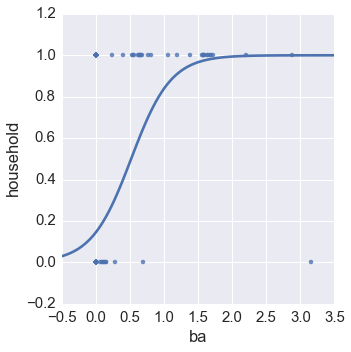
\includegraphics[width=0.4\linewidth]{glasslogsns}
% %\end{center}
% %\end{frame}
% %
% %%%%%%%%%%%%%%%%%%%%%%%%%%%%%%%%%%%%%%%%%%%%%%%%%%%%%%%%%%%%%%%%%%%%%%%%%
% %\begin{frame}[fragile]\frametitle{Using Logistic Regression with Categorical Features}
% %\begin{lstlisting}
% %# original (continuous) feature
% %sns.lmplot(x='ba', y='household', data=glass, ci=None, logistic=True)
% %\end{lstlisting}
% %\begin{center}
% %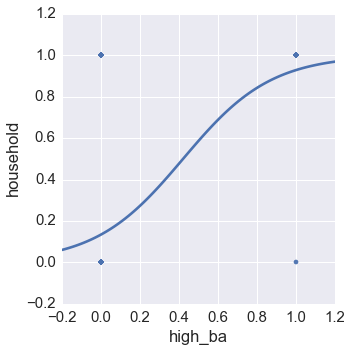
\includegraphics[width=0.5\linewidth]{glasslogsnscat}
% %\end{center}
% %\end{frame}
% %
% %%%%%%%%%%%%%%%%%%%%%%%%%%%%%%%%%%%%%%%%%%%%%%%%%%%%%%%%%%%%%%%%%%%%%%%%%
% %\begin{frame}[fragile]\frametitle{Using Logistic Regression with Categorical Features}
% %\begin{lstlisting}
% %# categorical feature, with jitter added
% %sns.lmplot(x='high_ba', y='household', data=glass, ci=None, logistic=True, x_jitter=0.05, y_jitter=0.05)
% %\end{lstlisting}
% %\begin{center}
% %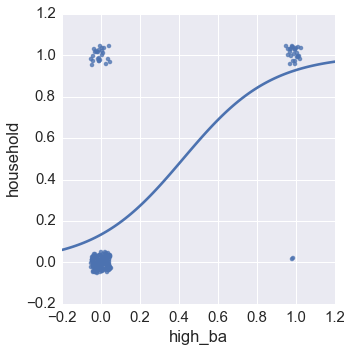
\includegraphics[width=0.5\linewidth]{glasslogsnscatjit}
% %\end{center}
% %\end{frame}
% %
% %%%%%%%%%%%%%%%%%%%%%%%%%%%%%%%%%%%%%%%%%%%%%%%%%%%%%%%%%%%%%%%%%%%%%%%%%
% %\begin{frame}[fragile]\frametitle{Using Logistic Regression with Categorical Features}
% %\begin{lstlisting}
% %# fit a logistic regression model
% %feature_cols = ['high_ba']
% %X = glass[feature_cols]
% %y = glass.household
% %logreg.fit(X, y)
% %
% %# examine the coefficient for high_ba
% %zip(feature_cols, logreg.coef_[0])
% %
% %[('high_ba', 4.4273153450187195)]
% %\end{lstlisting}
% %Interpretation: Having a high 'ba' value is associated with a 4.43 unit increase in the log-odds of 'household' (as compared to a low 'ba' value).
% %\end{frame}

% %%%%%%%%%%%%%%%%%%%%%%%%%%%%%%%%%%%%%%%%%%%%%%%%%%%%%%%%%%%%%%%%%%%%%%%%
% \begin{frame}[fragile]\frametitle{Comparing Logistic Regression with Other Models}
% Advantages of logistic regression:
% \begin{itemize}
% %\item Highly interpretable (if you remember how)
% \item     Model training and prediction are fast
% %\item     No tuning is required (excluding regularization)
% %\item     Features don't need scaling
% \item     Can perform well with a small number of observations
% %\item     Outputs well-calibrated predicted probabilities
% \end{itemize}
% Disadvantages of logistic regression:
% \begin{itemize}
% % \item 
% %    Presumes a linear relationship between the features and the log-odds of the response
% \item     Performance is (generally) not competitive with the best supervised learning methods
% %\item     Can't automatically learn feature interactions

% \end{itemize}
% \end{frame}


% %
% %%%%%%%%%%%%%%%%%%%%%%%%%%%%%%%%%%%%%%%%%%%%%%%%%%%%%%%%%%%%%%%%%%%%%%%%%
% %\begin{frame}[fragile]\frametitle{``Default.csv'' Dataset}
% %\begin{itemize}
% %\item 10,000 observations
% %
% %\item 4 variables
% %	\begin{itemize}
% %	\item Default: ${Yes, No}$ - whether customer defaulted on their debt
% %	\item Student: ${Yes, No}$ - whether customer is a student
% %	\item Balance: average CC balance
% %	\item Income: customer income
% %	\end{itemize}
% %
% %\item Considering Balance as feature and Default as outcome, $\beta_1 = 0.0047$
% %\end{itemize}
% %\begin{lstlisting}
% %reg = linear_model.LogisticRegression()
% %reg.fit(default['balance'].reshape(-1,1), default['default'])
% %Coefficients: [[ 0.00478248]]
% %Intercept: [-9.46506555] 
% %\end{lstlisting}
% %A one-unit increase in balance is associated with an increase in the log odds of default by 0.0047 units.
% %\end{frame}
% %
% %
% %
% %%%%%%%%%%%%%%%%%%%%%%%%%%%%%%%%%%%%%%%%%%%%%%%%%%%%%%%%%%%%%%%%%%%%%%%%%
% %\begin{frame}[fragile]\frametitle{Logistic Regression}
% %\begin{itemize}
% %\item Logistic regression is available in scikit-learn via the class \texttt{sklearn.linear\_model.LogisticRegression}. 
% %\begin{lstlisting}
% %from sklearn.linear_model import LogisticRegression
% %
% %est = LogisticRegression()
% %plot_datasets(est)
% %\end{lstlisting}
% %\end{itemize}
% %\end{frame}
% %
